% Comment 5: Interpretation of the Results: The authors argue that the effects on crime are driven primarily by geographic specialization, rather than additional resources, and leverage variation in the amount of additional resources across municipalities to provide evidence for their claim. However, it is unclear from the paper what drives the variation in additional resources. If municipalities experiencing larger increases in crime are those getting larger increases in resources, then this margin of exposure to the “resource channel” is endogenous. The paper may benefit from explaining what determines the variation in resources across municipalities and whether it correlates with trends in crime. As mentioned above, it may also help to provide more details on “Plan Cuadrante” such as whether it was accompanied by public information campaigns or media coverage, which could plausibly affect perceptions of security (one of their key outcomes) independently of actual crime rates (see Ajzenman et al. 2023 on this mechanism).

Thanks for the comment. Let us start by clarifying our main claim: we do not argue that the additional resources brought by \emph{Plan Cuadrante} have no effect on crime. Our key finding in the heterogeneity analysis by resource increases is that even municipalities that experienced no increase in resources relative to the control group show sizeable effects on nearly every outcome considered (see Figure \ref{fig:figure02}). In this context, where resource increases may be endogenous, we cannot rule out a role for resources in explaining the effects of \emph{Plan Cuadrante} in municipalities that received large increases, nor can we rule out that resources were important for the successful implementation of the beat policing component in those municipalities. However, the finding that municipalities with no additional resources relative to the control group still experience sizeable effects provides clear evidence that the beat policing component of the program plays an important independent role, which is our main point. Consistent with this, and in line with the revised manuscript, we now emphasize that these effects remain sizeable in municipalities with resource increases similar to those in control municipalities. We also find that subsequent increases in police resources outside \emph{Plan Cuadrante} have very limited effects on victimization. First, conditional on municipality and year fixed effects, changes in resources are not associated with reductions in crime. Second, we estimate the effect of a national program that increased police resources without any organizational component and find null effects on crime. Finally, the main estimates are robust to the inclusion of police resources as control variables, which, while by definition bad controls as they are themselves affected by \emph{Plan Cuadrante}, do not meaningfully alter the coefficients.


On what determined the size of the resource increases: During the 2000s and 2010s, the Chilean government substantially increased the overall number of Carabineros and other police resources such as patrol vehicles, and this increase benefited both treated and control municipalities. On top of this general trend, \emph{Plan Cuadrante} aimed to provide treated municipalities with sufficient additional resources to successfully implement the program. Panels (c) and (d) of Figure \ref{fig:figure05} show that, on average, \emph{Plan Cuadrante} substantially increased police resources relative to the control group. Panels (a) and (b) of Figure \ref{fig:figure_resources} show, however, that this increase masks substantial heterogeneity across treated municipalities: while municipalities in the bottom 40\% of the resource-increase distribution experienced increases very similar to those observed in control municipalities, municipalities in the top 40\% experienced substantially larger increases, with officers rising annually by around 22\% and patrol vehicles by around 80\% upon joining \emph{Plan Cuadrante}. So, what drives the variation in additional resources across treated municipalities? In principle, the goal was for \emph{Plan Cuadrante} to increase resources enough to cover each municipality's pre-existing resource deficit, measured in Equivalent Surveillance Units (UVEs). However, program documents make clear that budgetary constraints meant that all municipalities joined \emph{Plan Cuadrante} without fully closing this gap \citep{DIPRES2014, DIPRES2007_largo}, and program evaluations do not clearly establish that the size of this remaining deficit is what determined the resource increase each municipality received. We asked Carabineros for access to the official demand and supply figures that were supposed to guide this allocation, but this information was not provided. Importantly, we find that municipalities receiving larger versus smaller resource increases---whether the split is based on the increase in police officers or in patrol vehicles---do not display differential pre-treatment trends in either the outcomes of interest or in police resources themselves.\footnote{The p-values for the joint test of equal pre-trends between the two groups are, for the officers-based split and the patrol-vehicles-based split respectively: 0.823 and 0.048 for victimization, 0.059 and 0.379 for crime perception, 0.820 and 0.157 for investment in security measures, 0.213 and 0.419 for reported crime, 0.616 and 0.444 for police officers, and 0.405 and 0.157 for patrol vehicles.} We also explore the correlates of the resource increase in Online Appendix B, where we show that pre-treatment outcomes levels are not predictive of the size of the resource increase, while structural municipality characteristics such as population and poverty are more predictive.


Regarding the possibility that the effects on crime perception are driven by accompanying public information campaigns or media coverage, we believe this is unlikely for two reasons. First, \emph{Plan Cuadrante} was an internal operational reform of Carabineros with no formal public communication component in its design. While the program received some media attention when it was broadly rolled out across Santiago in 2000, we find no evidence of targeted information campaigns at the municipality level when individual municipalities subsequently joined the program, and the staggered rollout over more than a decade makes a sustained media salience mechanism implausible. Second, and more importantly, if the improvement in crime perception were driven by media coverage or information campaigns, one would expect the effects to be concentrated shortly after adoption and to fade over time. Instead, the dynamic estimates show that the effects on crime perception grow and persist over time, a pattern more consistent with a genuine improvement in security than with a transitory salience effect of the kind documented in \citet{Ajzenman_Pato}.

All these implementation details are provided in Section 2 in the updated manuscript, which expands substantially the section describing the implementation of \emph{Plan Cuadrante}:

\begin{adjustwidth}{2em}{0em}
{\setcounter{figure}{0}\renewcommand{\thefigure}{\arabic{figure}}
Carabineros, Chile's national police force, was founded in 1927. Through most of our study period, Carabineros operated under the Ministry of Defense, which oversaw both military and police functions until domestic security responsibilities were transferred to the Ministry of Interior in 2011.\footnote{Currently, Carabineros reports to the Ministry of Public Security, created in 2024 to focus exclusively on domestic security.}

Carabineros' mission, functions, and structure are established by Law 18.961 and the Regulation on Carabineros' Organization (Reglamento de Carabineros) \citep{Ley18961,ReglamentoCarabineros1989}. Under this framework, Carabineros is a professional, disciplined, and hierarchical police institution whose mission is to preserve public order and security with a central emphasis on preventive policing. The General Director heads the strategic level, responsible for defining doctrine and institutional strategy, while the Subdirector coordinates implementation. The Directorate of Order and Security administers police functions at the tactical level.

Territorially, Carabineros is organized into zones that oversee \emph{prefecturas}. Zones and \emph{prefecturas} are primarily management layers. Zones map roughly one-to-one to Chile's regional divisions, with two exceptions: the Metropolitan Region of Santiago---the most populated in the country---and La Araucanía---which has recently experienced significant social conflict---are each divided into two zones. Each zone is subdivided into \emph{prefecturas}---54 nationwide---which supervise 227 \emph{comisar\'ias}, the main operational units at the tactical level. These \emph{comisar\'ias} oversee smaller units---\emph{subcomisar\'ias}, \emph{tenencias}, \emph{retenes}, \emph{puestos}, and \emph{avanzadas}---that operate within their assigned jurisdictions.\todo{JORGE: Since we need to cut on the manuscript, I believe this paragraph is a good candidate to be removed or shortened.}

In practice, the \emph{comisar\'ia} is the basic unit of routine frontline policing and, in most municipalities, serves as the territorial anchor of police work. Officers conduct patrol, surveillance, prevention, and first response at this level. In most municipalities, a single \emph{comisar\'ia} covers the entire municipal territory, though larger municipalities may have multiple ones. Santiago, for instance, has four. %By contrast, 112 municipalities---mostly remote or rural---have no \emph{comisar\'ia} and are served through smaller subordinate posts linked to a \emph{comisar\'ia}. 
All municipalities that adopted \emph{Plan Cuadrante} during our study period had a \emph{comisar\'ia}. With the exception of 9 municipalities, each had a single \emph{comisar\'ia} covering the full municipal territory. On average, a \emph{comisar\'ia} in our sample covered 1,608 square kilometers and served 57,642 inhabitants. %Of these, 17 had no subordinate units, whereas the remaining 79 had between one and nine.

\emph{Plan Cuadrante} was introduced within this institutional framework without altering Carabineros' hierarchical structure or its strategic and tactical levels. The reform emerged in a context of rising victimization and insecurity, with the explicit goal of reversing these trends \citep{PCSP2014}. Its central innovation was a shift toward a beat policing model. In the criminology literature, beat policing refers to assigning officers to fixed territorial areas so they can accumulate local knowledge, strengthen ties with residents, and respond more effectively to local crime patterns \citep{cordner1995community,skogan1997comminuty}. In practice, the catchment area of police forces in municipalities adopting \emph{Plan Cuadrante} was partitioned into smaller, fixed geographic units (quadrants), to which officers were permanently assigned. Rather than building new infrastructure, the reform redefined the territorial responsibility of officers in already existing police stations \citep{DIPRES2007_largo}.\footnote{In 2016, Carabineros launched the \emph{Plan Cuadrante 2.0} program in those municipalities served by \emph{Plan Cuadrante}. While this reform introduced additional reforms aimed at integrating the community into the provision of security and building capacity to gather and analyze crime data in police stations, this paper's study period ends before these improvements were introduced.} This represented a clear break from the pre-reform system, in which officers rotated across broad operational territories, very often spanning entire municipalities.

Carabineros began piloting \emph{Plan Cuadrante} in 1998. The program expanded gradually through 2013, as shown in Panel (a) of Figure \ref{fig:figure01}, reaching 150 urban municipalities and covering roughly 90\% of Chile's population.\footnote{Further details about the expansion of \emph{Plan Cuadrante} are provided in Online Appendix \ref{sec:appendixA} and Table \ref{tab:implementation}.} Online Appendix A provides further details about the rollout of the program. The rollout was designed to follow a municipality ranking based on a weighted index of victimization, police resource deficits, drug prevalence, unemployment, and demand for police services, with annual entry determined by available budget.\footnote{The weights assigned to each component changed on a yearly basis \citep{DIPRES2007_largo,DIPRES2014}.} In practice, however, Budget Office evaluations show that adoption diverged from this ranking for undocumented reasons, so the rule operated more as a loose guideline than as a binding assignment mechanism \citep{DIPRES2014}.

\FloatBarrier
%--- Implementation
\begin{figure}[h!]
    \centering
    \caption{Implementation of \emph{Plan Cuadrante}}
    \label{fig:figure01}
    \begin{subfigure}{0.58\textwidth}
        \centering
        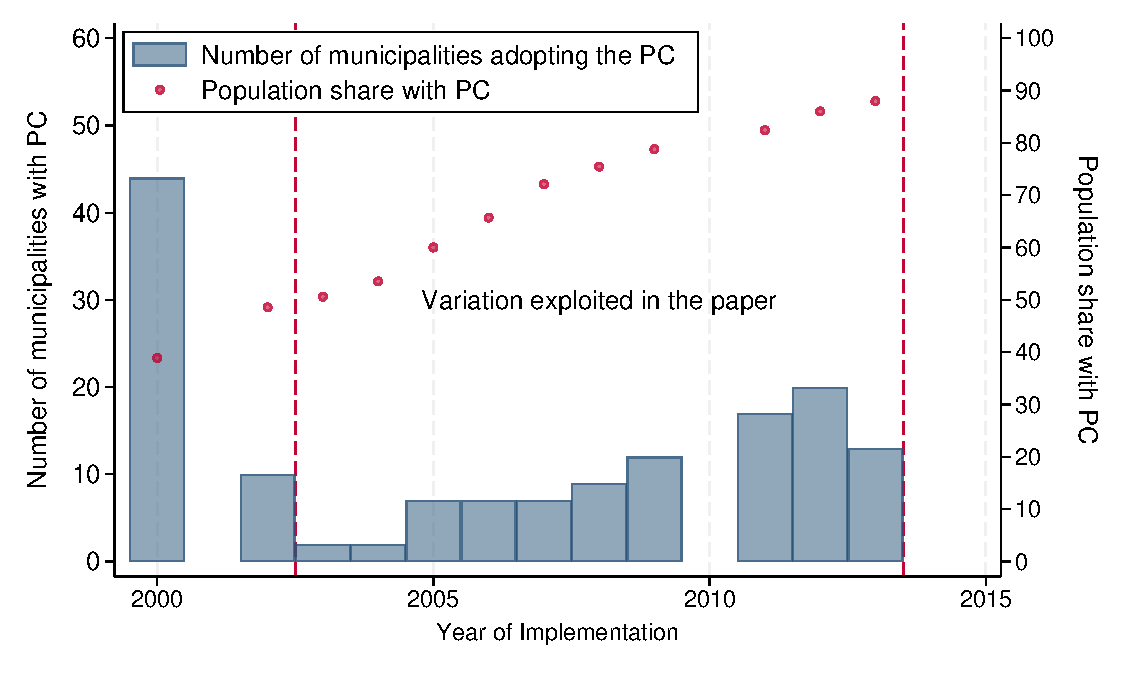
\includegraphics[width=1\textwidth]{../manuscript/Graphs/Graph_PCvariation.pdf}
        \caption{Adoption of \emph{Plan Cuadrante}}
    \end{subfigure}
    \\
    \begin{subfigure}{\textwidth}
    \centering
    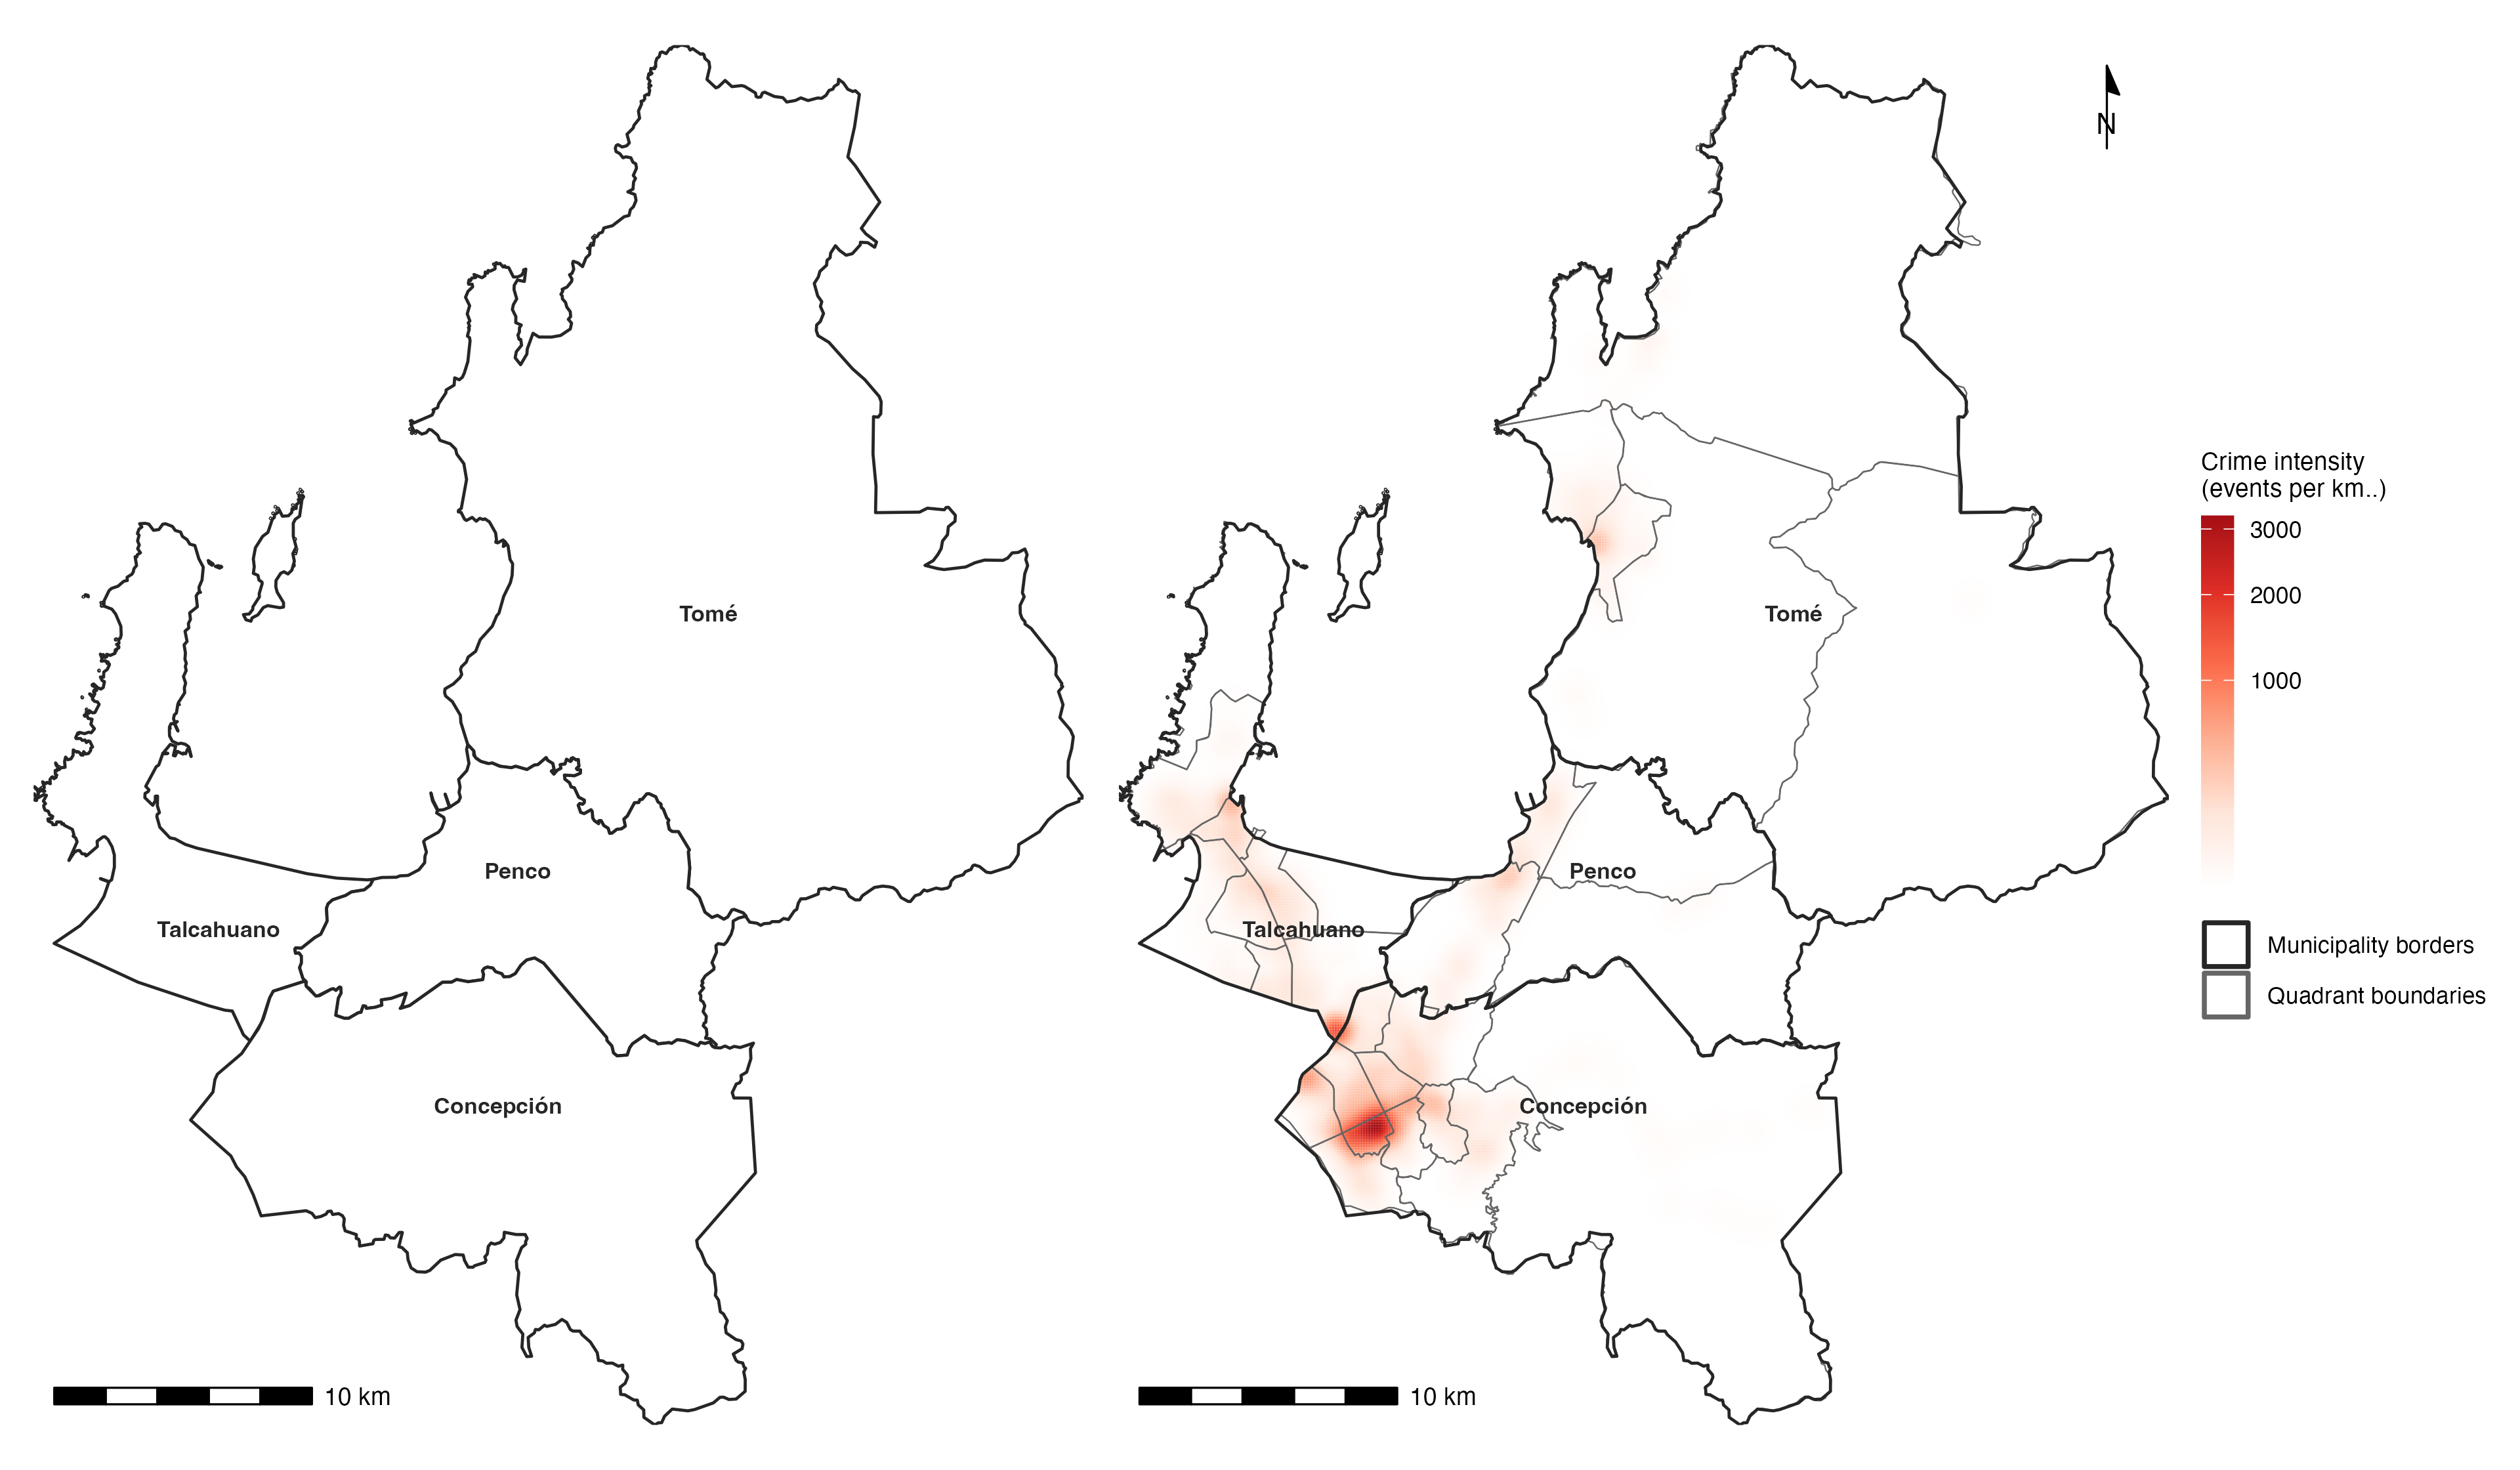
\includegraphics[width=0.65\linewidth]{../manuscript/Graphs/Graph_PCexample_combined.png}
    \caption{\emph{Plan Cuadrante} in the Concepci\'on area}
    \end{subfigure}%
 %   \\
 %   \begin{subfigure}{0.58\textwidth}
 %       \centering
 %       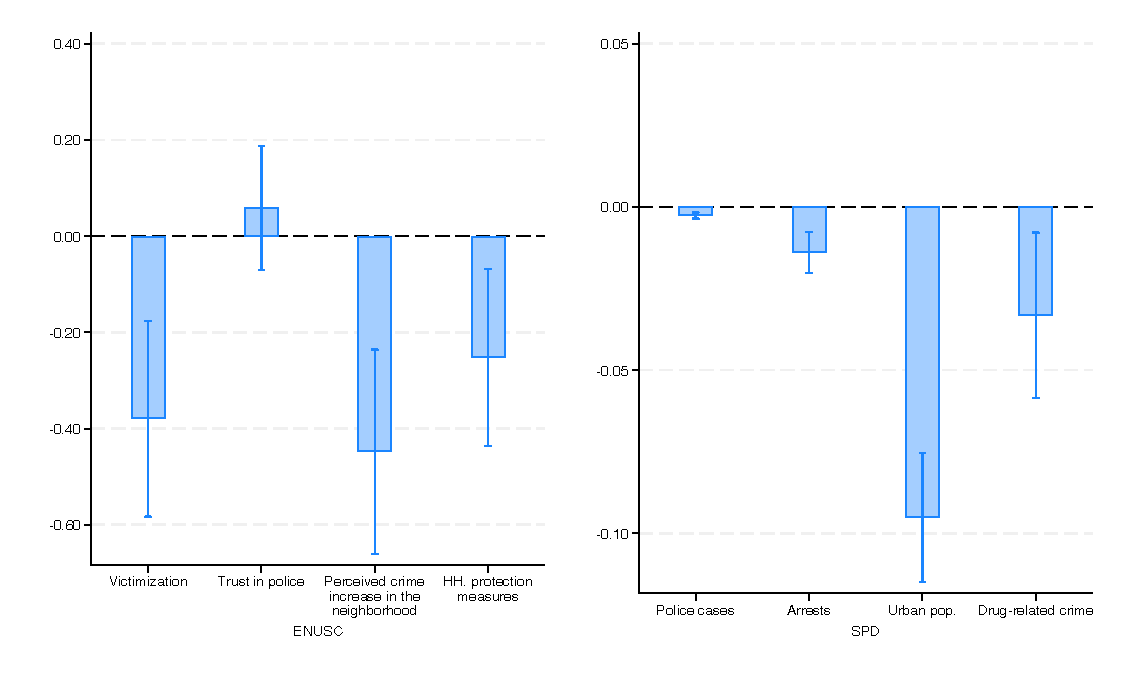
\includegraphics[width=1.1\textwidth]{../manuscript/Graphs/results_predictorsPC_combined.pdf}
 %       \caption{Time of Adoption and Municipality Characteristics}
  %  \end{subfigure}%
    \\[12pt]
    \begin{minipage}{0.95\textwidth}
    \footnotesize Notes: Panel (a) shows the number of municipalities adopting the \emph{Plan Cuadrante} each year (bars), while the circles above them illustrate the cumulative share of the Chilean population living in a municipality with the \emph{Plan Cuadrante} already in place. Panel (b) depicts the metropolitan area of Concepci\'on, the second-largest in Chile: the left map shows its four municipalities---the original police catchment areas---and the right map overlays the Carabineros quadrants together with a kernel-density estimate of all types of robberies and thefts recorded by the police (both reported crimes and arrests). It illustrates how \emph{Plan Cuadrante} subdivided each catchment area (which corresponds to the territory of a municipality) into smaller quadrants, as well as the spatial concentration of crime within them.
    \end{minipage}
\end{figure}
\clearpage

\FloatBarrier

Conceptually, police effectiveness can be viewed as a function of three inputs: total resources, territorial deployment, and policing strategy. Although in some municipalities police resources were increased significantly to operationalize the beat policing model \citep{DIPRES2007_largo,DIPRES2014}, the program primarily transformed the latter two elements. The creation of quadrants was accompanied by permanent geographic assignment of officers to specific areas. This change was operationally critical. By making officers responsible for their quadrant, it encouraged accumulation of local knowledge and stronger community ties, allowing them to adapt patrols and prevention activities to local crime patterns. Importantly, this was not driven by program-specific operational directive changes. Throughout the period we study, a single national set of operational guidelines applied to officers in both treated and control municipalities \citep{Manual_Carabineros2018,DIPRES2007_largo}. Thus, while the average effects we document on crime and crime perception likely reflect combined changes in the three elements we discuss---i.e., resources, deployment, and strategy---the deployment change itself was essential to operationalizing the reform. We discuss the drivers of the effects we document in Section \ref{mechanisms}.

Quadrant size and shape were determined by local police authorities based on factors such as road networks, geographic features, and available resources. In principle, resource allocation across quadrants followed demand for police services, measured in Equivalent Surveillance Units (UVEs); in practice, the station commander retained discretionary authority, as was also the case prior to \emph{Plan Cuadrante} \citep{DIPRES2014}. Municipalities implementing \emph{Plan Cuadrante} were subdivided into an average of seven quadrants, each typically staffed by approximately three officers per shift. On average, each quadrant covered 185 square kilometers and served 13,466 inhabitants. Panel (b) of Figure \ref{fig:figure01} illustrates this structure, showing the 29 quadrants created across the four municipalities of the Concepción metropolitan region---Chile's second-largest metropolitan area and the largest in our sample. Quadrants represented approximately 14\% of the original \emph{comisar\'ia} territory. Officers continued to operate from the same police station but were permanently assigned to a specific sub-area within its jurisdiction. While Carabineros' hierarchical structure limits frontline officer decision-making authority, each quadrant was assigned a Quadrant Delegate (\textit{Delegado de Cuadrante}), a non-commissioned officer, responsible for immediate operational decisions within the quadrant.

\emph{Plan Cuadrante} may affect public safety through two complementary channels: deterrence and police effectiveness, understood as the capacity to respond to and resolve crimes. The changes induced by \emph{Plan Cuadrante}---permanently assigning officers to well-defined neighborhoods and, in some municipalities, increasing available resources---can increase both police visibility and local knowledge. As officers repeatedly patrol the same area, they become familiar with its streets, residents, and routines, which can raise the perceived probability of identification and apprehension and reduce the expected returns to crime. At the same time, this deeper knowledge of local territory and communities can improve police response and case resolution once crimes occur. The reform therefore likely affects both dimensions. Consistent with this interpretation, in Section \ref{results} we document declines in victimization and in reported crime---patterns consistent with deterrence---together with increases in arrests, consistent with improved police effectiveness.

Although beat policing shares features with other policing approaches, such as hot-spot policing and community-based policing, which have been widely studied, it has distinctive features that make it worth studying as an independent approach. Hot-spot policing concentrates resources in high-crime areas and does not focus on building local knowledge and community ties. It is typically implemented through targeted interventions at specific locations rather than systematic territorial organization, and the same officers are not necessarily sent repeatedly to the same areas. Evidence on hot-spot policing is mixed, with some studies showing crime reductions in targeted areas but also potential displacement effects \citep{SR_1}. \emph{Plan Cuadrante}, by contrast, subdivided all urban municipalities into quadrants with permanent officer assignment. As Panel (b) of Figure \ref{fig:figure01} illustrates, some quadrants contained crime hot-spots, but many did not. The reform thus addressed entire urban territories rather than specific high-crime areas, potentially mitigating displacement effects associated with hot-spot policing.

Community-based policing emphasizes building relationships with residents and addressing underlying social issues, and typically involves active community participation in defining strategy and priorities---in some cases, even assuming surveillance and prevention responsibilities. While increasing trust in the police and strengthening community ties were among the declared goals of \emph{Plan Cuadrante}, and may have resulted from its territorial reorganization, the community was not formally involved in the provision of security.\footnote{The \emph{Plan Cuadrante}'s original design contemplated a formal community integration model (MICC) with a Community Affairs Office (\textit{Oficina de Asuntos Comunitarios}) and a dedicated officer in each police station. However, this model was not implemented during our study period. Independent program evaluations from the Budget Office document that these Community Affairs Offices did not exist and had no dedicated personnel, budget, or structured activities in the period we study \citep{DIPRES2007_largo,DIPRES2014}. The community integration model was piloted in four police stations during 2012--2013, none of which are in our analytical sample. Financing was then discontinued in early 2014 and only restored and expanded after our study period ends.}%
 %Similarly, Operations Offices (\textit{Oficina de Operaciones}) formally assigned crime analysis functions but relied on paper-based entry systems, lacking digital infrastructure, analysts, or centralized data systems throughout the study period \citep{DIPRES2014}. Both the community integration model and crime analysis function were substantively implemented only with \emph{Plan Cuadrante} 2.0 (2015--2017) \citep{Carabineros2018}, outside our study period.}

In recent decades, police departments worldwide have transitioned toward beat policing reforms \citep{NASEM2018,PCSP2014}, yet the effectiveness of this model has not been rigorously assessed. Although the beat policing approach introduced through \emph{Plan Cuadrante} shares features with programs previously studied in the economic literature, its distinctive characteristics---comprehensive territorial reorganization and systematic local officer specialization---make it a valuable case for studying how deployment and policing strategies not yet examined in the economics literature affect crime and crime perception.

}
\end{adjustwidth}

We also include below Section 4.4, which summarizes the analyses disentangling the role of resources from that of the beat policing component discussed above:\\

\begin{adjustwidth}{2em}{0em}
{\setcounter{figure}{3}\renewcommand{\thefigure}{\arabic{figure}}
%\textbf{4.4 What Is Driving the Effects of \emph{Plan Cuadrante}?}


To reduce crime and improve security perceptions, police forces need to strengthen both prevention and police effectiveness. Both margins can be shaped by resources, territorial deployment, and policing strategy. This section examines which components of \emph{Plan Cuadrante} are most likely to drive the effects documented in Section \ref{results}. 

The central objective of \emph{Plan Cuadrante} was to introduce a beat policing model by reorganizing deployment. Police operational territories that had typically matched municipal boundaries were subdivided into quadrants, and officers were permanently assigned to these quadrants. During our study period, national operational guidelines remained the same in adopting and non-adopting municipalities. Still, this new deployment likely affected policing strategy at a more operational level, because it allowed officers to adapt patrol routes, schedules, and prevention practices using the local knowledge that the program sought to build.

Although changes in resources were not the core of the reform, implementation contemplated increases in municipalities that lacked the personnel and patrol capacity required to move to this model. During the period we study, Chile was expanding public spending on security, and police resources increased in most municipalities regardless of whether or when they adopted \emph{Plan Cuadrante}. On average, however, municipalities adopting the program experienced larger increases in officers and patrol vehicles, as shown in panels (a) and (b) of Figure \ref{fig:resources}. Since increases in police resources have been shown to reduce crime in some contexts \citep{Evans}, this pattern raises a central question for interpretation, namely whether our estimates reflect resource expansion or the deployment and strategy changes introduced by \emph{Plan Cuadrante}. We address this question through a set of exercises that exploit heterogeneity in resource increases across municipalities and over time.

\FloatBarrier
%--- Implementation
\begin{figure}[H]
    \centering
    \caption{Plan Cuadrante and Changes in Police Resources}
    \label{fig:resources}
    \label{fig:figure_resources}
    \begin{tabular}{cc}
        \begin{minipage}[t]{0.48\textwidth}
            \centering
            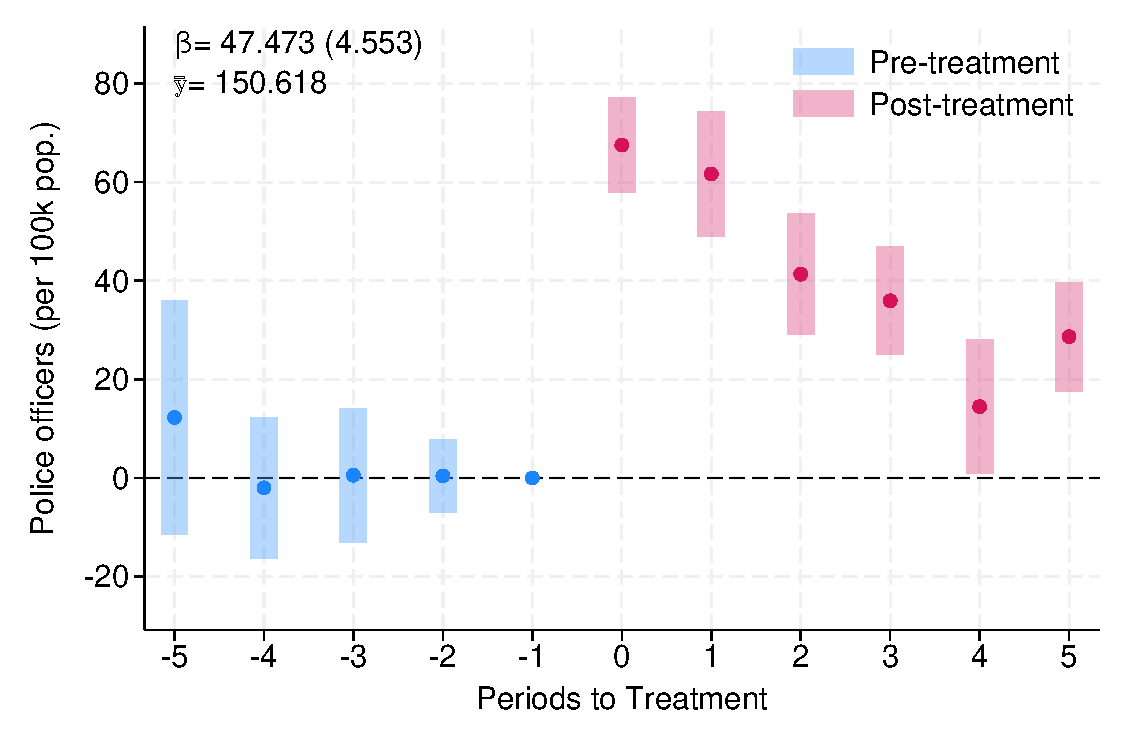
\includegraphics[width=\linewidth]{../manuscript/Graphs/fig4_officers.pdf}

            \small (a) Effect on the number of police officers
        \end{minipage}
        &
        \begin{minipage}[t]{0.48\textwidth}
            \centering
            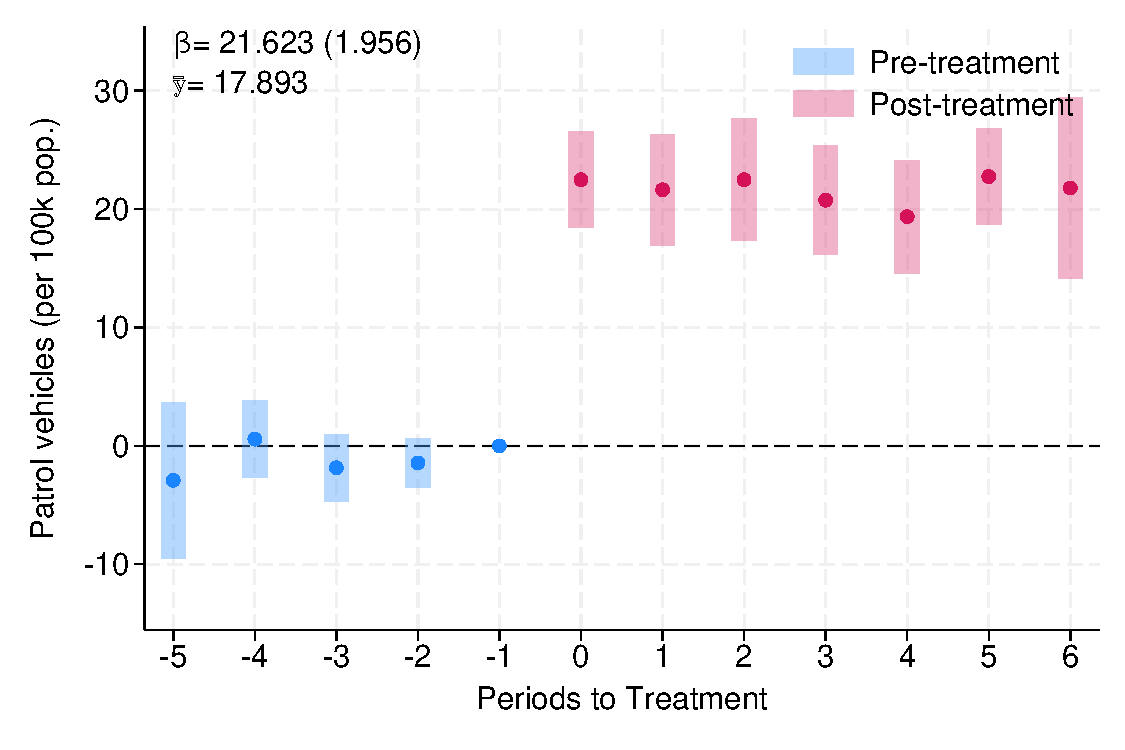
\includegraphics[width=\linewidth]{../manuscript/Graphs/fig4_patrols.pdf}

            \small (b) Effect on the number of patrol vehicles
        \end{minipage}
        \\[4pt]
        \begin{minipage}[t]{0.48\textwidth}
            \centering
            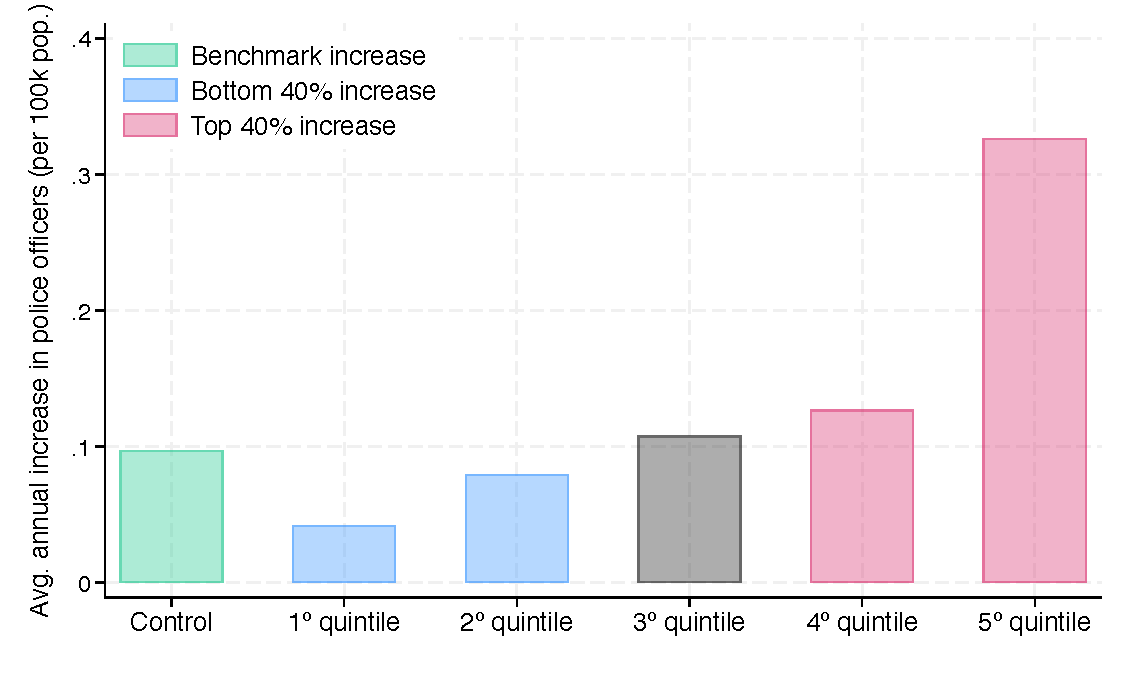
\includegraphics[width=\linewidth]{../manuscript/Graphs/increase_enusc_off_quintiles.pdf}

            \small (c) Distribution of $\Delta$ in police officers
        \end{minipage}
        &
        \begin{minipage}[t]{0.48\textwidth}
            \centering
            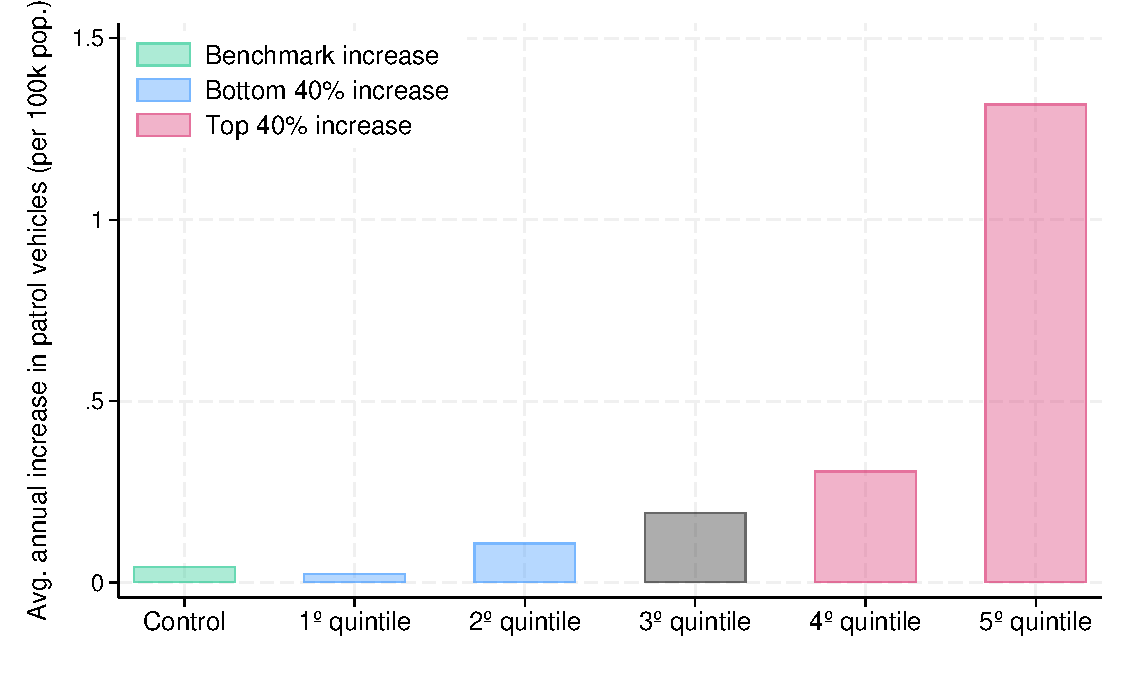
\includegraphics[width=\linewidth]{../manuscript/Graphs/increase_enusc_pv_quintiles.pdf}

            \small (d) Distribution of $\Delta$ in patrol vehicles
        \end{minipage}
        \\[4pt]
        \begin{minipage}[t]{0.48\textwidth}
            \centering
            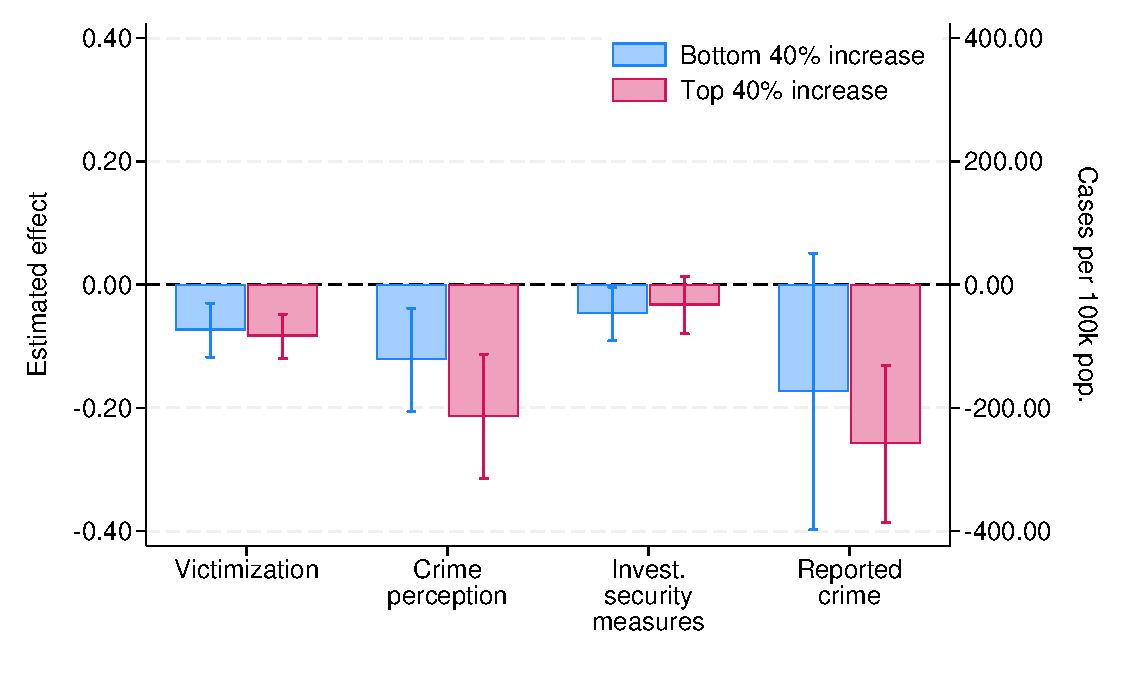
\includegraphics[width=\linewidth]{../manuscript/Graphs/heterogeneity_off.pdf}

            \small (e) Effects by the intensity of $\Delta$ in police officers
        \end{minipage}
        &
        \begin{minipage}[t]{0.48\textwidth}
            \centering
            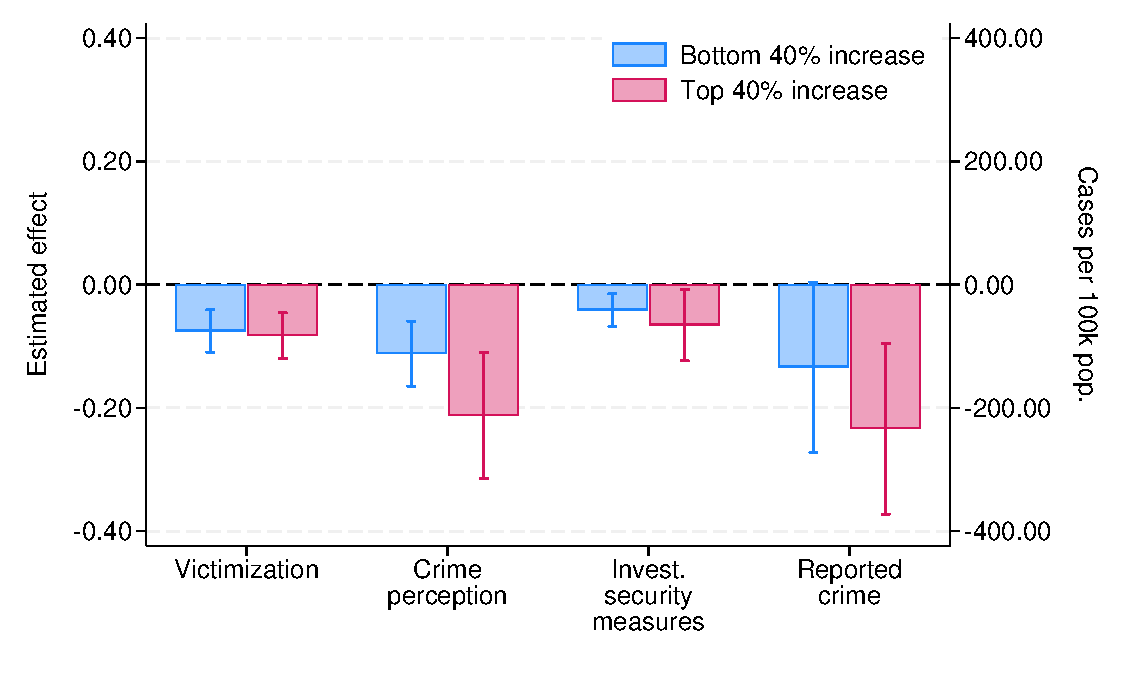
\includegraphics[width=\linewidth]{../manuscript/Graphs/heterogeneity_pv.pdf}

            \small (f) Effects by the intensity of $\Delta$ in patrol vehicles
        \end{minipage}
    \end{tabular}
    \vspace{4pt}
    \begin{minipage}{0.99\textwidth}
    \footnotesize Notes: Panels (a) and (b) show the effect of \emph{Plan Cuadrante} on police officers and patrol vehicles per 100,000 inhabitants. Panels (c) and (d) show the distribution of annual changes in officers and patrol vehicles across municipalities. Panels (e) and (f) report effects by the intensity of resource changes, comparing municipalities in the bottom 40\% and top 40\% of the distribution. The estimation follows \citet{Callaway}. The graphs display estimated coefficients and 95\% confidence intervals. Standard errors are clustered at the municipality level using wild bootstrapping.
    \end{minipage}
\end{figure}
\FloatBarrier
Panels (c) and (d) of Figure \ref{fig:resources} show that the average increase in police resources masks substantial heterogeneity. Municipalities in the bottom 40\% of the resource-change distribution (blue bars) experienced increases close to the average annual variation observed among never treated and not-yet-treated municipalities (green bar). By contrast, municipalities in the top 40\% (red bars) experienced much larger increases, with officers rising by around 22\% and patrol vehicles by around 80\%. If the effects of \emph{Plan Cuadrante} were driven by resource increases alone, we would not expect effects in municipalities whose resource increases were similar to those of the control group. Yet panels (e) and (f) of Figure \ref{fig:resources} show sizeable effects for most crime and crime-perception outcomes even in that low-increase group. While there may be a resource gradient for some crime-perception outcomes, the effects on twelve-month victimization and private investment in security among municipalities with control-like resource increases are close in magnitude to those in municipalities with larger increases. Reassuringly, municipalities in the top and bottom 40\% of the resource-increase distribution do not display differential pre-treatment trends in outcomes or police resources, which suggests that this heterogeneity is not driven by differential pre-existing trends.\footnote{We test for the joint significance of the pre-treatment coefficients between the two groups, separately for the split based on the increase in police officers and the split based on the increase in patrol vehicles. The resulting p-values are, respectively, 0.823 and 0.048 for victimization, 0.059 and 0.379 for crime perception, 0.820 and 0.157 for investment in security measures, and 0.213 and 0.419 for reported crime, as well as 0.616 and 0.444 for police officers and 0.405 and 0.157 for patrol vehicles.}

Although we cannot fully separate the beat policing component from the resource component of the reform---resources may have been important to enable effective implementation of the program, or may explain part of the effects in some municipalities---the fact that municipalities with resource increases similar to those experienced by control municipalities still display sizeable effects indicates that the effects of \emph{Plan Cuadrante} are not driven entirely by resources.\footnote{We also re-estimate the results in Figure \ref{fig:figure02} but controlling for police resources. Online Appendix Table \ref{tab:results_controlbyresources} shows that the magnitude of the estimated effects remains similar for most variables, although the statistical significance is reduced in some estimations. This likely reflects a mechanical feature of the \citet{Callaway} estimation procedure: control variables are not incorporated parametrically, but are instead used to construct the comparison group via outcome regression or propensity-score weighting, so the resulting estimation uncertainty propagates to the ATT standard errors. Note, in addition, that police resources are a bad control---i.e., at least part of their variation is a result of the adoption of \emph{Plan Cuadrante}---so these results should be interpreted cautiously.}\footnote{Table \ref{tab:resourcecorrelates} in Online Appendix \ref{sec:appendixB} examines which factors are associated with a larger increase in police resources upon the adoption of \emph{Plan Cuadrante}.}


\FloatBarrier
%--- Implementation
\begin{figure}[h!]
    \centering
    \caption{Police Resources and Public Safety}
    \label{fig:resources2}
    \begin{subfigure}[t]{0.55\textwidth}
        \centering
        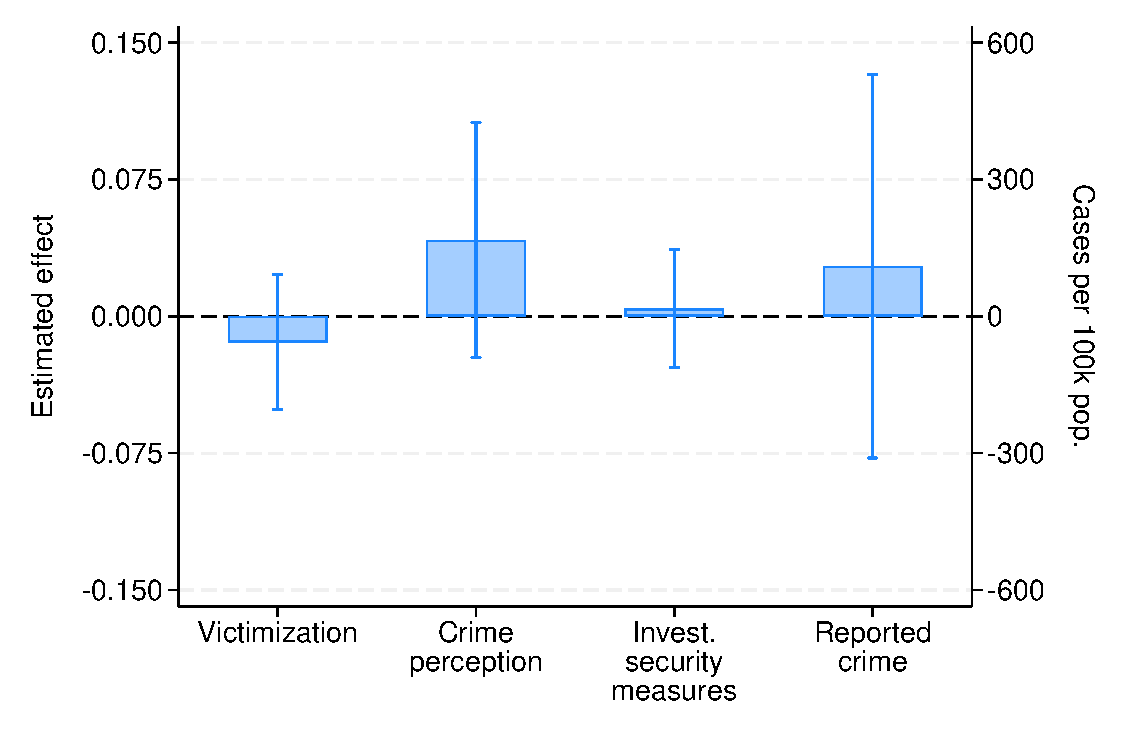
\includegraphics[width=\linewidth]{../manuscript/Graphs/results_SC_att_combined.pdf}
        \caption{Effects of \emph{Seguridad Ciudadana}}
    \end{subfigure}
    \\[6pt]
    \begin{subfigure}[t]{0.55\textwidth}
        \centering
        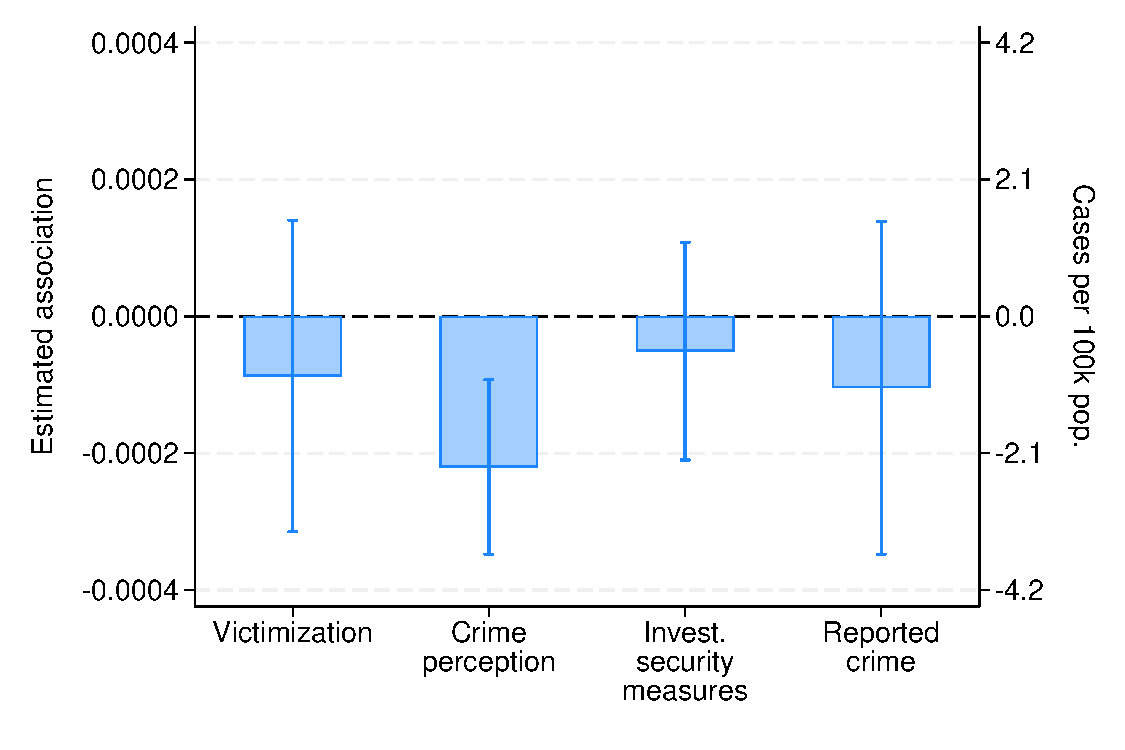
\includegraphics[width=\linewidth]{../manuscript/Graphs/results_corr_novariation_off_santiago.pdf}
        \caption{Association between police officers and effectiveness}
    \end{subfigure}
    \\[6pt]
    \begin{subfigure}[t]{0.55\textwidth}
        \centering
        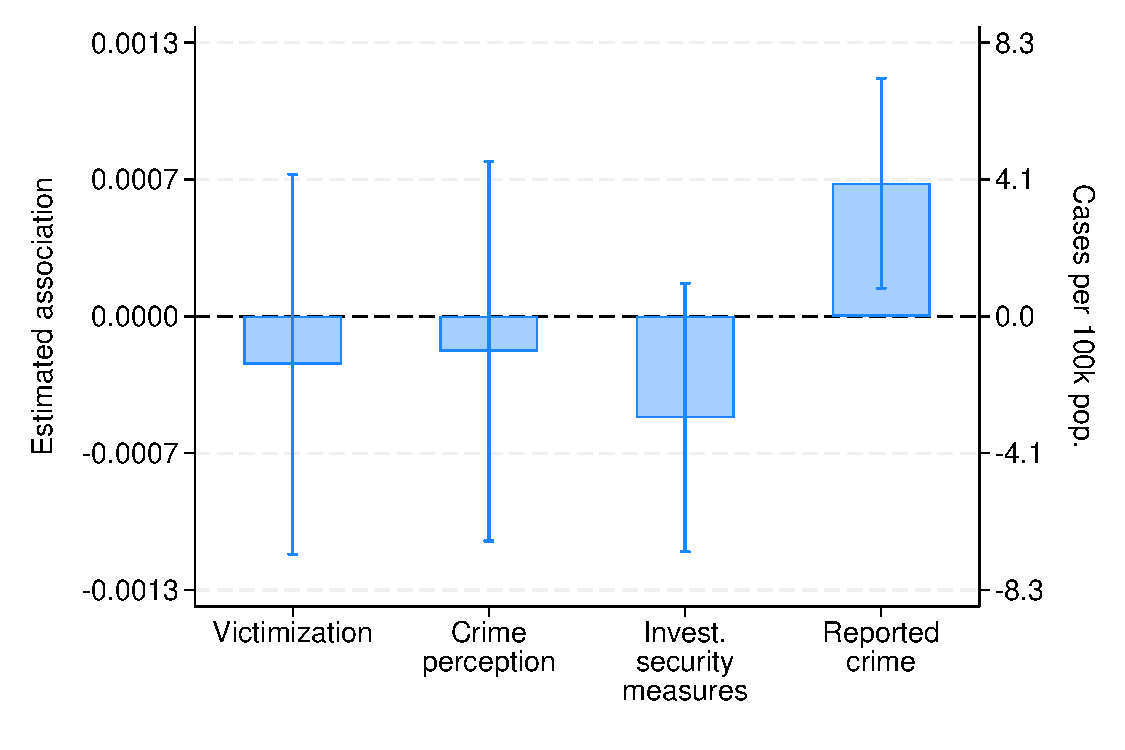
\includegraphics[width=\linewidth]{../manuscript/Graphs/results_corr_novariation_veh_santiago.pdf}
        \caption{Association between patrol vehicles and effectiveness}
    \end{subfigure}
    \\[8pt]
    \begin{minipage}{0.99\textwidth}
    \footnotesize Notes: Panel (a) reports the pooled effect of \emph{Seguridad Ciudadana}, a program that expanded local security personnel to support patrolling and deterrence but did not replicate the deployment-and-strategy features of \emph{Plan Cuadrante}. Panels (b) and (c) report within-municipality associations between police resources and police-effectiveness outcomes among the 41 municipalities of the Santiago Metropolitan Region, all of which had adopted \emph{Plan Cuadrante} by 2000. The regressions include municipality and year fixed effects. Standard errors are clustered at the municipality level using the wild bootstrapping procedure.
    \end{minipage}
\end{figure}
\FloatBarrier

To further investigate whether resource increases alone can explain our results, we assess the effects of \emph{Seguridad Ciudadana}, a program that expanded local security personnel to support patrolling and deterrence, but did not replicate the core deployment-and-strategy features of \emph{Plan Cuadrante}. Using a difference-in-differences specification following \citet{Callaway}, panel (a) of Figure \ref{fig:resources2} shows no significant effects of these resource changes on police effectiveness. Further details about this exercise and the corresponding event-study estimates are reported in Online Appendix \ref{sec:appendixB} and Online Appendix Figure \ref{fig:figureA5}. 


Finally, we study whether variation in police resources in municipalities that had already adopted \emph{Plan Cuadrante} improves public safety and security perceptions. Using ENUSC data and information on resources for 2006--2012 in the 41 municipalities of the Santiago Metropolitan Region---all of which had adopted \emph{Plan Cuadrante} by 2000---we exploit variation in officers and patrol vehicles that is unrelated to program adoption. Panels (b) and (c) of Figure \ref{fig:resources2} show the association between police resources and our main outcomes, conditional on municipality and year fixed effects. With one exception---the association between police officers and crime perception---none of these associations is statistically significant at conventional confidence levels. \footnote{Online Appendix Figure \ref{fig:figureA7B} reports the same exercise and also shows similar results for the broader set of municipalities that adopted \emph{Plan Cuadrante} before 2006 and never-treated municipalities (red bars); see Online Appendix \ref{sec:appendixB} for further details.}

Taken together, these results suggest that resource increases alone do not account for the effects of \emph{Plan Cuadrante}. We next turn to evidence that speaks more directly to the beat-policing components of the reform.

Panel (a) of Figure \ref{fig:police_performance} shows that, following the adoption of \emph{Plan Cuadrante}, households are much more likely to report increased police presence in their neighborhoods. The share of households perceiving increased police presence rises by 35 percentage points (156\%), the share reporting that police pass by their house daily rises by 22 percentage points (59\%), the share reporting never seeing police patrols near their house falls by 10 percentage points (57\%), and complaints about lack of police surveillance fall by around 5 percentage points (20\%). This evidence is consistent with both larger resources and the new deployment model. Yet the latter estimate---the only police-presence outcome for which we can separately estimate effects in municipalities with small and large resource increases---is similar in magnitude across the two groups, which suggests that the increase in police presence is not explained only by larger resource increases (see Online Appendix Figure \ref{fig:heterogeneity_appendix}).\footnote{We cannot estimate heterogeneous effects for other police-presence outcomes, such as the reporting of police passing by or the share of households perceiving an increase in police presence, because those variables are available only in ENUSC rounds 2003, 2005, and 2006, while resource data start in 2006.} More importantly, the broader pattern of results suggests that \emph{Plan Cuadrante} did more than simply increase patrolling intensity. Existing work shows that police presence can reduce crime while officers are present, but that its overall effects may be attenuated when crime is displaced across places or time windows \citep{MASTROBUONI2019, Blanes_Mastrobuoni_2018}. Our results point to something broader. As discussed in Section \ref{results}, we find actual declines in victimization and reported crime, together with no evidence of spillovers to neighboring municipalities. This pattern is more consistent with officers accumulating local knowledge and adapting prevention strategies to local conditions under stable territorial assignment than with a purely mechanical increase in patrol intensity.

Panel (b) of Figure \ref{fig:police_performance} reinforces this interpretation. Households in early-adopting municipalities report better police performance across multiple dimensions. They are 8.1 percentage points (16\%) more likely to rate police performance as good or very good, 7.6 percentage points (11\%) more likely to describe police as efficient, 5 percentage points (6\%) more likely to report that police are helpful, and 4.9 percentage points (7\%) more likely to report that police are well informed. They are also 3.9 percentage points (10\%) less likely to perceive police as corrupt, 7.9 percentage points (21\%) less likely to believe police fail to control crime, and 7.6 percentage points (22\%) less likely to report that police do not perform their duties effectively.\footnote{Information on police performance is only available in ENUSC round 2005. Using this round, we compare perceived police performance in municipalities that adopted \emph{Plan Cuadrante} in 2005 or earlier and in municipalities adopting after 2005. Figure \ref{fig:balance_doseresponse} in Online Appendix \ref{sec:appendixB} shows that the number of years of exposure to \emph{Plan Cuadrante} is positively correlated with perceived police performance. While these exercises on perceived police performance should be interpreted with caution, we show in the same appendix that the timing of future adoption is not correlated with perceived police performance in 2005 for municipalities that had not yet adopted the program by 2005.} %These perceived improvements are consistent with a setting in which officers become better informed about local routines and more effective in how they patrol and respond.

The administrative evidence points in the same direction. Panel (c) of Figure \ref{fig:police_performance} shows that arrests per 100,000 inhabitants increase by 48 (14\%) in our main estimates, even as crime declines overall.\footnote{As with reported crime, this event study is restricted to 5 pre-treatment and 7 post-treatment periods for symmetry with the ENUSC-based analysis; Online Appendix Figure \ref{fig:admin_uncapped} reports the results for arrests using the full set of pre-treatment and post-treatment periods.} This effect is also significant among municipalities with resource increases similar to those in the control group (see Online Appendix Figure \ref{fig:heterogeneity_appendix}). Consistent with this pattern, panel (d) of Figure \ref{fig:police_performance} shows that the arrest rate per reported crime also increases by 1.7 percentage points (10\%), suggesting that a higher share of crimes reported to the police are being solved. Because these gains appear even where resources did not increase more than in control municipalities, they are difficult to reconcile with a pure resource story and are more naturally interpreted as improvements in police effectiveness under the deployment and strategy changes introduced by \emph{Plan Cuadrante}. The corresponding event-study estimates for arrests, the arrest rate per reported crime, and trust in the police in Figure \ref{fig:police_performance} confirm that these changes emerge only after adoption.

Finally, panel (e) of Figure \ref{fig:police_performance} shows a sharp increase in trust in the police in our main specification (Section \ref{results}), consistent with one of the objectives of beat policing, namely bringing officers closer to the community and allowing them to accumulate local knowledge through repeated interaction. Online Appendix Figure \ref{fig:heterogeneity_appendix} shows that this effect remains sizeable both in municipalities that experienced resource increases similar to the control group and in those with larger increases.

Overall, although resources were likely important for implementation and may explain part of the effects in some municipalities, the results in this section indicate that resource changes alone are not enough to explain our findings. The evidence is more consistent with a combination of deployment changes and the strategy adjustments enabled by local knowledge accumulation under permanent assignment to quadrants.

\FloatBarrier
%--- Implementation
\begin{figure}[!ht]
    \centering
    \caption[\emph{Plan Cuadrante} and Changes in Police Performance]{\emph{Plan Cuadrante} and Changes in Police Performance}
    \label{fig:figure05}
    \label{fig:police_performance}
    \label{fig:effectiveness_es}
    \begin{subfigure}[t]{0.44\textwidth}
        \centering
        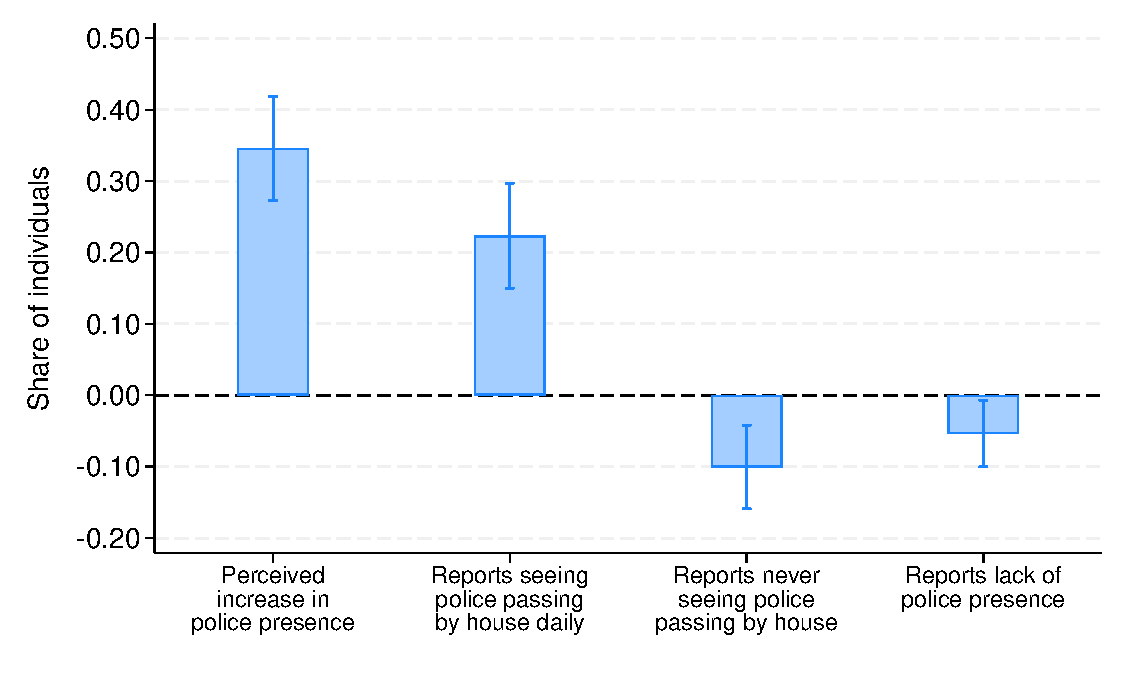
\includegraphics[width=\linewidth]{../manuscript/Graphs/results_policepresence.pdf}
        \caption{Effect on police presence}
    \end{subfigure}\hfill
    \begin{subfigure}[t]{0.44\textwidth}
        \centering
        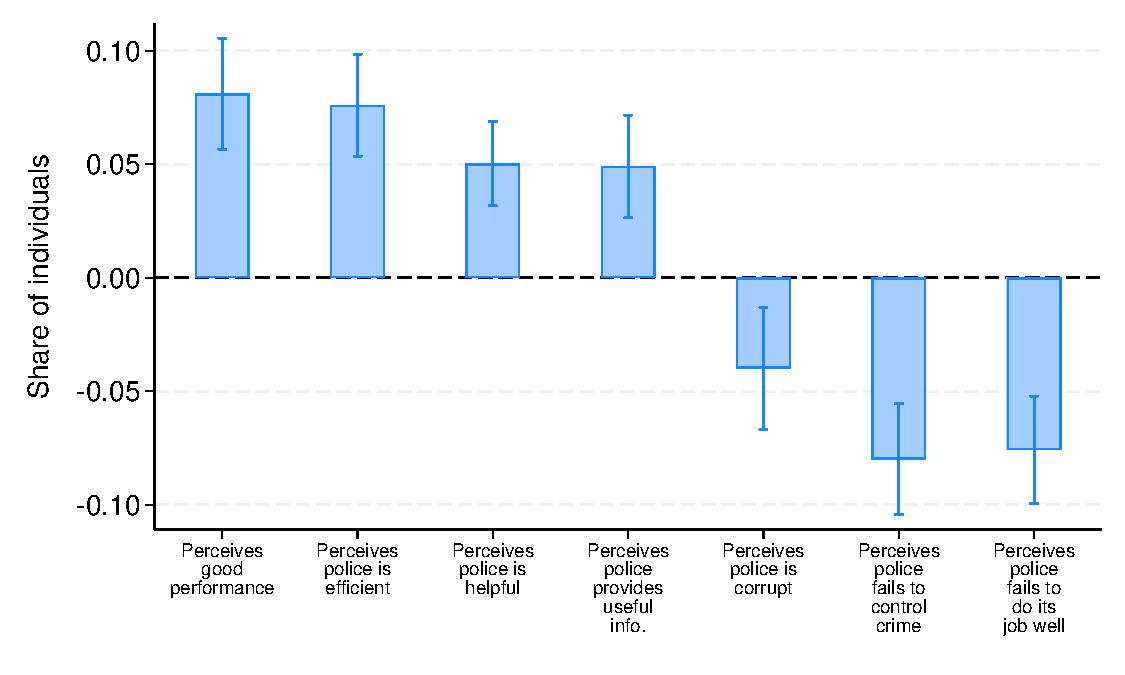
\includegraphics[width=\linewidth]{../manuscript/Graphs/combined_PCttest_2.pdf}
        \caption{Effect on perceived police performance}
    \end{subfigure}
    \\[6pt]
    \begin{subfigure}[t]{0.44\textwidth}
        \centering
        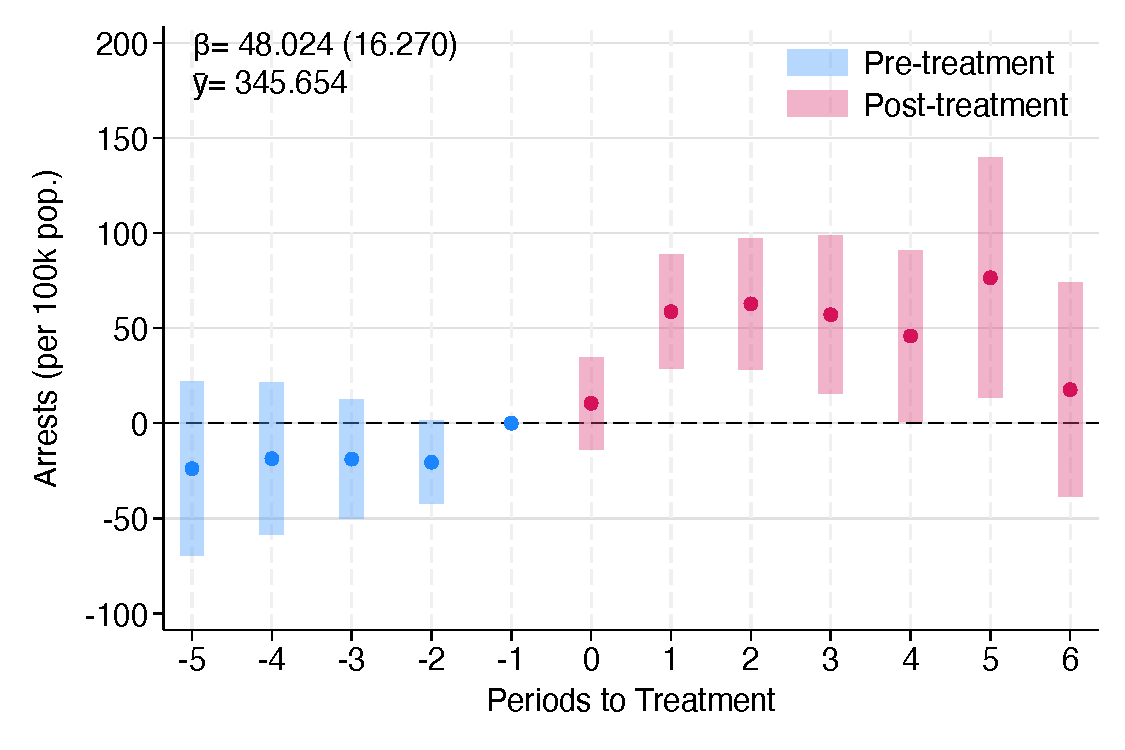
\includegraphics[width=\linewidth]{../manuscript/Graphs/totalarrestscrime_allcomunas.pdf}
        \caption{Arrests (per 100k pop.)}
    \end{subfigure}\hfill
    \begin{subfigure}[t]{0.44\textwidth}
        \centering
        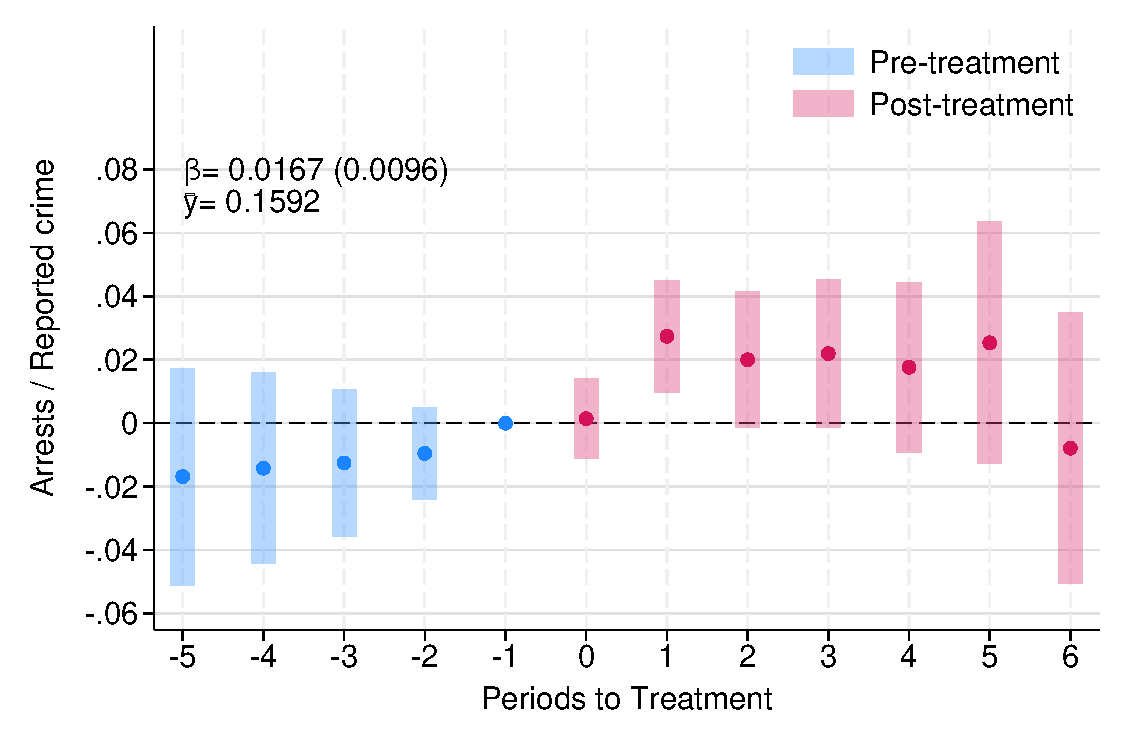
\includegraphics[width=\linewidth]{../manuscript/Graphs/arrests_over_reportedcrime_allcomunas.pdf}
        \caption{Arrests / Reported crime}
    \end{subfigure}
    \\[6pt]
    \begin{subfigure}[t]{0.44\textwidth}
        \centering
        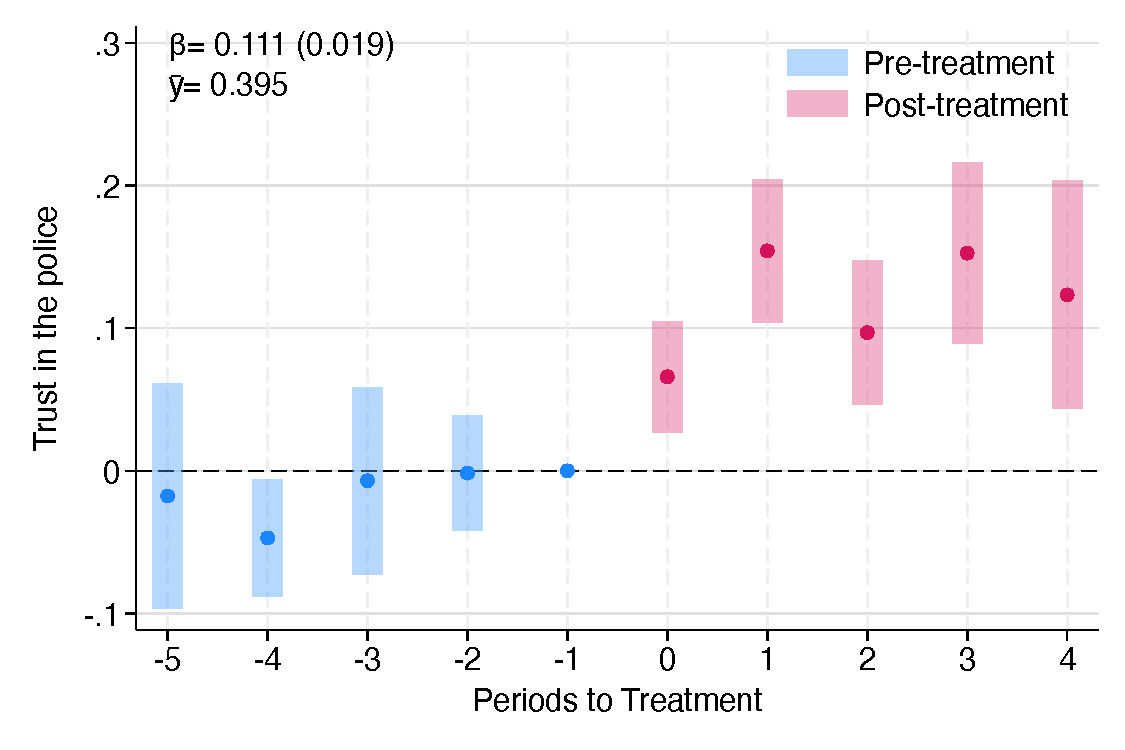
\includegraphics[width=\linewidth]{../manuscript/Graphs/results_trustcarabineros.pdf}
        \caption{Trust in the police}
    \end{subfigure}
    \\[8pt]
    \begin{minipage}{0.99\textwidth}
    \footnotesize Notes: Panel (a) reports the effects on perceived police presence. Panel (b) reports perceived police performance in 2005, comparing municipalities where \emph{Plan Cuadrante} was already implemented before 2006 with municipalities where it was implemented after 2005. Panels (c), (d), and (e) report dynamic event-study estimates for arrests per 100,000 inhabitants, the ratio of arrests to reported crime, and trust in the police. The estimation follows \citet{Callaway}. The graphs display estimated coefficients and 95\% confidence intervals. Standard errors are clustered at the municipality level using the wild bootstrapping procedure.
    \end{minipage}
\end{figure}

\FloatBarrier

%Overall, while resources were arguably important for implementation, the evidence suggests that the beat policing elements---permanent assignment of officers to quadrants and greater local knowledge---were important drivers of the improvements in public safety and security perceptions we document in the paper.



 
}
\end{adjustwidth}

We also added a new Online Appendix B subsection, ``Factors Associated with the Increase in Police Resources,'' regressing the increase in resources at the time of adoption on pre-treatment municipality characteristics. Because the UVE demand-and-supply files were not provided by \textit{Carabineros}, we cannot infer the exact administrative rule used to assign the additional resources:

\begin{adjustwidth}{2em}{0em}
As discussed in Section \ref{institutions} and in Online Appendix \ref{resources_plan_cuadrante}, the increase in police resources associated with the adoption of \emph{Plan Cuadrante} varied substantially across municipalities. In principle, this increase should be related to each municipality's pre-existing police resource deficit---measured in Equivalent Surveillance Units (UVEs)---which \emph{Plan Cuadrante} was meant to help close. However, program evaluations do not clearly establish that this deficit is what determined the size of the resource increase each municipality received \citep{DIPRES2007_largo,DIPRES2014}.\footnote{Although we requested information on the demand and supply of UVEs underlying this allocation, this information was not provided by \textit{Carabineros}.} If the pre-existing deficit is not what determines the resource increase, what is it related to? Reassuringly, municipalities receiving larger versus smaller resource increases do not display differential pre-treatment trends in either the outcomes of interest or in police resources themselves.\footnote{We test for the joint significance of the pre-treatment coefficients between the two groups, separately for the split based on the increase in police officers and the split based on the increase in patrol vehicles. The resulting p-values are, respectively, 0.823 and 0.048 for victimization, 0.059 and 0.379 for crime perception, 0.820 and 0.157 for investment in security measures, and 0.213 and 0.419 for reported crime, as well as 0.616 and 0.444 for police officers and 0.405 and 0.157 for patrol vehicles.} In this section we examine whether the magnitude of the resource increase experienced by a municipality upon adoption is correlated with its pre-treatment levels in crime, police resources, and other observable characteristics. Specifically, we regress the increase in resources at the time of adopting \emph{Plan Cuadrante} on municipality characteristics measured before the program's introduction, including crime and police resources in 2006, the first year for which information on police resources is available. Thus, we restrict this analysis to municipalities that adopted \emph{Plan Cuadrante} from 2007 onward.

Table \ref{tab:resourcecorrelates} reports OLS regressions of the average annual increase in police officers and patrol vehicles per 100,000 inhabitants on pre-adoption municipality characteristics, separately for the administrative (SPD) sample at the municipality level (columns 1--2) and the ENUSC sample at the survey-respondent level (columns 3--4). All variables are standardized and standard errors are clustered by municipality, so coefficients are comparable in magnitude across regressors.

The results provide little support for the hypothesis that municipalities with worse pre-treatment crime outcomes received systematically larger resource increases. Pre-treatment reported crime is, if anything, negatively associated with the subsequent increase in both officers and vehicles in the administrative sample (columns 1--2); in the ENUSC sample, it is negatively associated with the increase in officers (column 3), although it is positively associated with the increase in vehicles (column 4). Pre-treatment victimization is, if anything, negatively associated with both increases in the ENUSC sample (columns 3--4). Pre-treatment arrests, crime perception, trust in the police, and private investment in security measures are not significantly associated with the resource increase. The increase in resources is instead more strongly predicted by structural municipality characteristics: less populous municipalities experienced larger increases in three of the four specifications, and municipalities with higher poverty rates predicted a larger increase in vehicles in the administrative sample (column 2), although this association is not significant for officers in that sample (column 1) or in the ENUSC sample (columns 3--4).
\end{adjustwidth}

\clearpage
\noindent\textbf{Other figures and tables referenced above:}
\vspace{0.5em}

{\setcounter{figure}{1}\renewcommand{\thefigure}{\arabic{figure}}
%--- Implementation
\begin{figure}[h!]
    \centering
    \caption{Effects of \emph{Plan Cuadrante} on Crime Outcomes and Security Perceptions}
    \label{fig:figure02}
    \begin{subfigure}{0.495\textwidth}
        \centering
        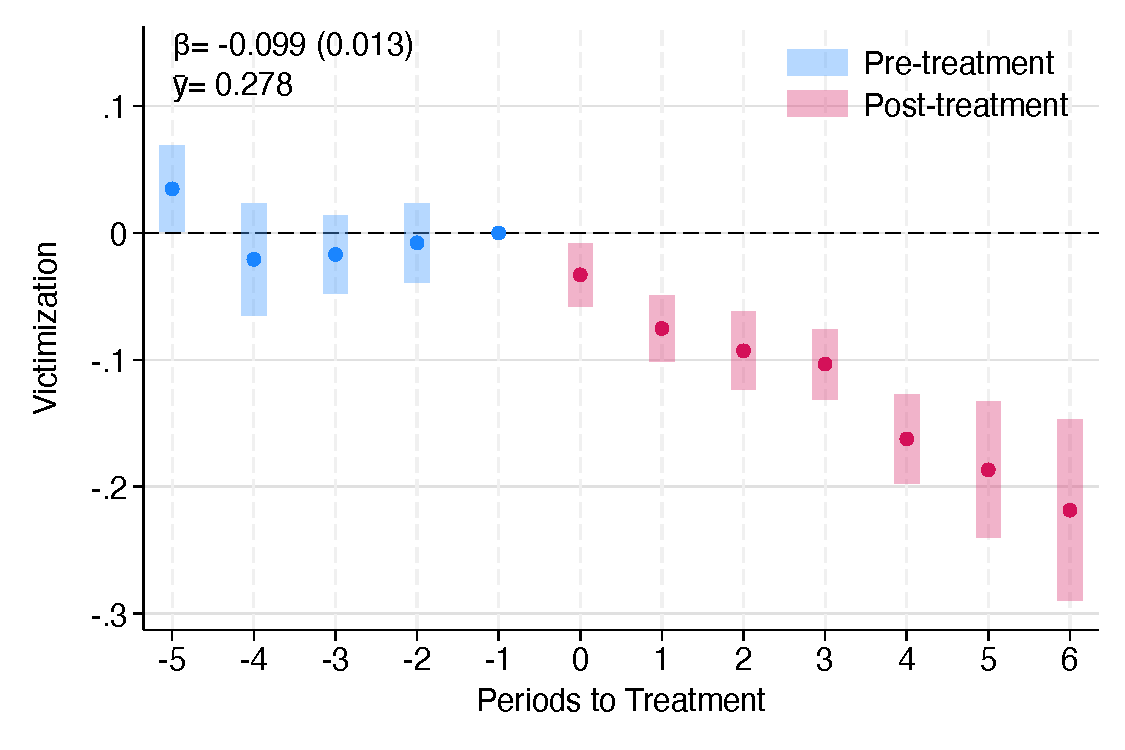
\includegraphics[width=\textwidth]{../manuscript/Graphs/results_victimization.pdf}
        \caption{Victimization in last 12 months}
    \end{subfigure}%
    ~
    \begin{subfigure}{0.495\textwidth}
    \centering
    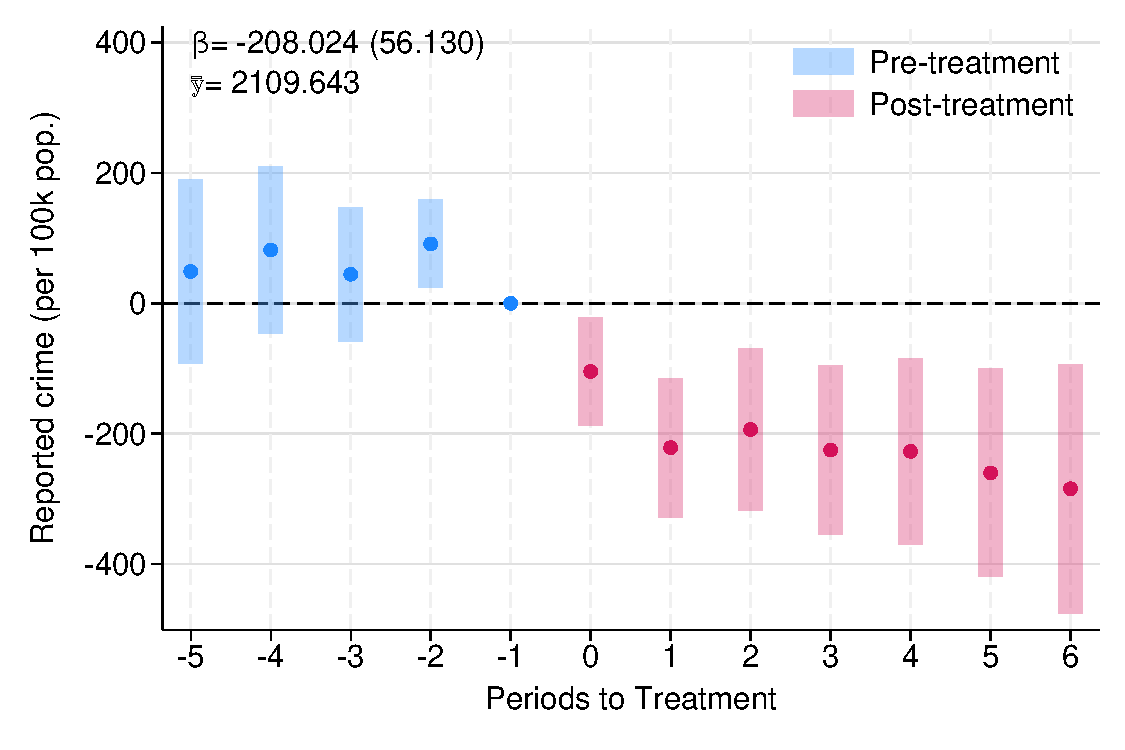
\includegraphics[width=\textwidth]{../manuscript/Graphs/totalreportedcrime_allcomunas.pdf}
        \caption{Reported crime per 100k inhabitants}
    \end{subfigure}
        \begin{subfigure}{0.495\textwidth}
        \centering
        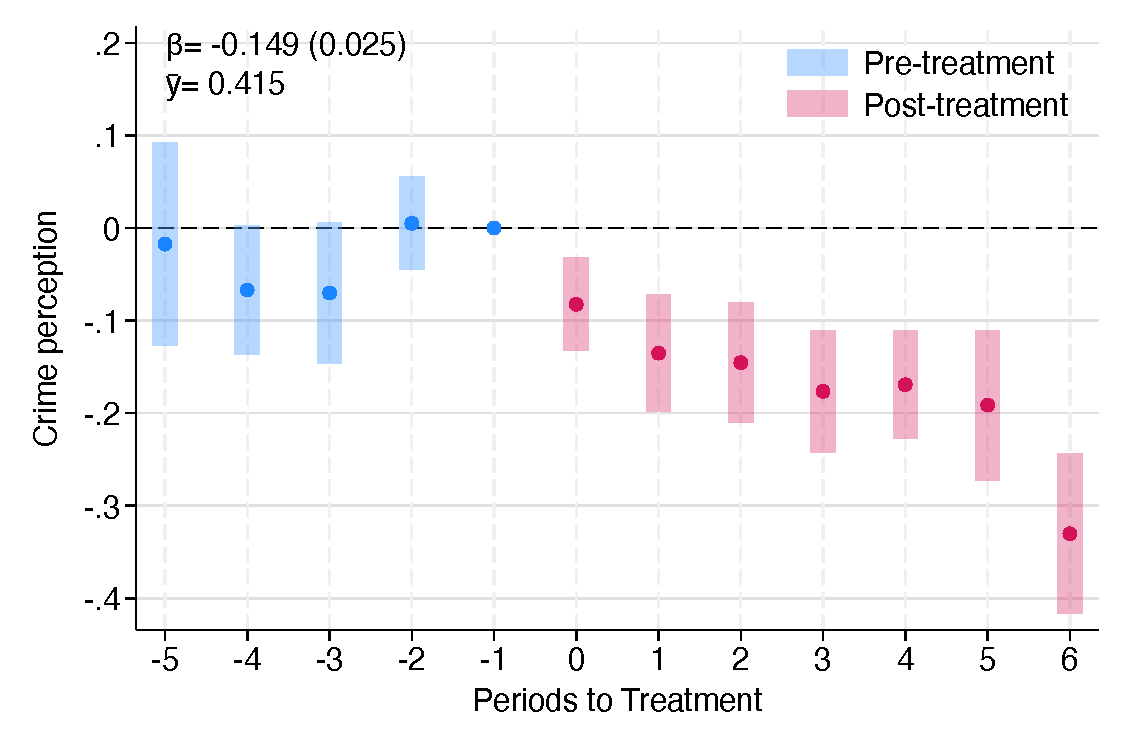
\includegraphics[width=\textwidth]{../manuscript/Graphs/results_perception.pdf}
        \caption{Households reporting an increase in crime}
    \end{subfigure}%
    ~
    \begin{subfigure}{0.495\textwidth}
    \centering
    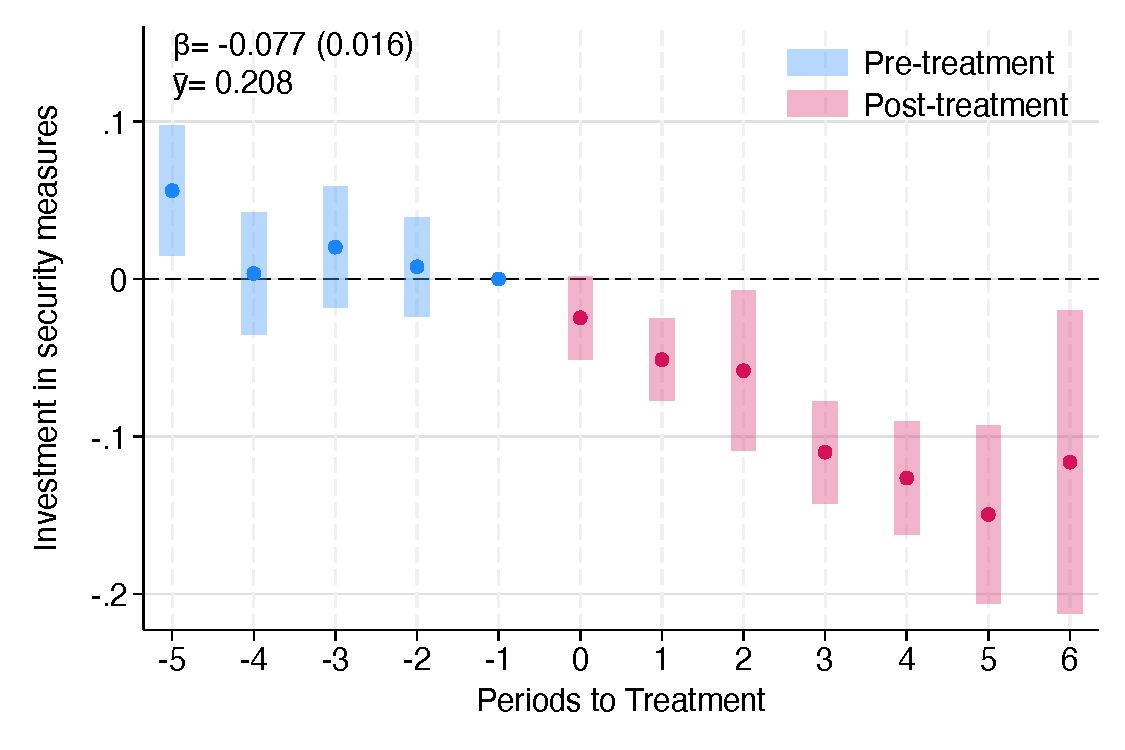
\includegraphics[width=\textwidth]{../manuscript/Graphs/results_hhprotectionmeasures.pdf}
        \caption{Households adopting security measures}
    \end{subfigure}
    \\[12pt]
    \begin{minipage}{0.99\textwidth}
    \footnotesize
    Notes: This figure shows the dynamic effects of the \emph{Plan Cuadrante} on different measures of police effectiveness. The estimation is conducted using the procedure developed in \citet{Callaway} for difference-in-differences with staggered treatment adoption. The dots in the figure represent the estimated coefficients and the bars behind them 95\% confidence intervals. Standard errors are clustered at the municipality level using the wild bootstrapping procedure. The pooled effect and the mean outcome before the introduction of the treatment is also presented in each panel. Panel (a) reports the effect of \emph{Plan Cuadrante} on the probability of household victimization in the last 12 months using the ENUSC survey. Panel (b) reports the effect on the number of crimes reported to the police in the municipality per 100,000 inhabitants using administrative data. Panel (c) reports the effect on the probability of perceiving an increase in crime using the ENUSC survey. Panel (d) reports the effect on the probability of adopting security measures in the last twelve months using the ENUSC survey. Panel (a) includes 93,041 observations; panel (b), 4,231; panel (c), 89,578; and panel (d), 93,041 observations.
    \end{minipage}
\end{figure}
}

\clearpage

{\renewcommand{\thetable}{B.4}
\begin{table}[H]
\centering
\caption{Predictors of the Increase in Police Resources under \emph{Plan Cuadrante}}
\label{tab:resourcecorrelates}
\begin{threeparttable}
\small
\setlength{\tabcolsep}{6pt}
\renewcommand{\arraystretch}{1.1}
\begin{tabular}{@{}l cc cc@{}}
\toprule
& \multicolumn{2}{c}{Administrative sample} & \multicolumn{2}{c}{ENUSC sample} \\
\cmidrule(lr){2-3} \cmidrule(lr){4-5}
& Police & Patrol & Police & Patrol \\
Dep.\ var: avg.\ annual increase & officers & vehicles & officers & vehicles \\
in resources (share of pre-adoption level) & (1) & (2) & (3) & (4) \\
\midrule
Reported crime (per 100k pop.) & $-0.203^{**}$ & $-0.199^{**}$ & $-0.319^{*}$ & $0.272^{*}$ \\
 & (0.099) & (0.097) & (0.182) & (0.137) \\
Arrests (per 100k pop.) & $0.099$ & $-0.041$ & $0.003$ & $0.297$ \\
 & (0.136) & (0.129) & (0.186) & (0.223) \\
Victimization &  &  & $-0.017^{*}$ & $-0.025^{*}$ \\
 &  &  & (0.010) & (0.013) \\
Crime perception &  &  & $0.005$ & $0.008$ \\
 &  &  & (0.017) & (0.014) \\
Trust in the police &  &  & $0.024$ & $0.027$ \\
 &  &  & (0.018) & (0.019) \\
Investment in security measures &  &  & $0.004$ & $-0.003$ \\
 &  &  & (0.010) & (0.009) \\
Police officers (per 100k pop.) & $-0.207$ & $0.155$ & $-0.888^{***}$ & $0.571^{***}$ \\
 & (0.155) & (0.129) & (0.154) & (0.136) \\
Patrol vehicles (per 100k pop.) & $-0.129$ & $-0.139$ & $0.537^{**}$ & $-0.507^{***}$ \\
 & (0.129) & (0.126) & (0.212) & (0.169) \\
Log population & $-0.529^{***}$ & $-0.203^{*}$ & $-0.193$ & $-0.626^{**}$ \\
 & (0.145) & (0.112) & (0.189) & (0.269) \\
Poverty rate (2004) & $0.170$ & $0.308^{**}$ & $0.027$ & $-0.017$ \\
 & (0.113) & (0.126) & (0.108) & (0.108) \\
\midrule
Observations & 65 & 65 & 8,781 & 8,781 \\
R-squared & 0.342 & 0.282 & 0.614 & 0.545 \\
\bottomrule
\end{tabular}
\begin{tablenotes}[flushleft]
\footnotesize
\item \textit{Note:} OLS regressions of the average annual increase in police officers (columns 1 and 3) and patrol vehicles (columns 2 and 4) per 100{,}000 inhabitants, from the year before adoption of \emph{Plan Cuadrante} to 2012. As in panels (a) and (b) of Figure \ref{fig:figure_resources}, the increase is expressed as a share of the resources available the year before adoption. Columns 1--2 use the administrative sample at the municipality level; columns 3--4 use ENUSC survey respondents interviewed before 2007 (survey outcomes at the respondent level, other regressors as pre-2006 municipality aggregates). All variables are standardized. Standard errors clustered by municipality in parentheses.
\item $^{*}p<0.1$; $^{**}p<0.05$; $^{***}p<0.01$.
\end{tablenotes}
\end{threeparttable}
\end{table}
}

\clearpage


